\documentclass[11pt]{article}
\usepackage[margin=1in]{geometry}
\usepackage{amsmath,amssymb}
\usepackage{booktabs}
\usepackage{graphicx}
\usepackage{array}
\usepackage{listings}
\usepackage{xcolor}
\usepackage[hidelinks]{hyperref}
\usepackage{caption}

\newcommand{\bx}{\mathbf{x}}
\newcommand{\bw}{\mathbf{w}}
\newcommand{\R}{\mathbb{R}}

\lstset{
  basicstyle=\ttfamily\small,
  breaklines=true,
  frame=single,
  columns=fullflexible,
}

\begin{document}

\begin{center}
{\Large\bfseries CSCI3230 / ESTR3108 2026--27 First Term Assignment 2}
\end{center}

\medskip
\noindent\fbox{\begin{minipage}{\dimexpr\linewidth-2\fboxsep-2\fboxrule}
{\itshape I declare that the assignment here submitted is original except for source material explicitly acknowledged, and that the same or closely related material has not been previously submitted for another course. I also acknowledge that I am aware of University policy and regulations on honesty in academic work, and of the disciplinary guidelines and procedures applicable to breaches of such policy and regulations, as contained in the following websites.}

\smallskip
University Guideline on Academic Honesty:\\
\url{http://www.cuhk.edu.hk/policy/academichonesty/}\\
Faculty of Engineering Guidelines to Academic Honesty:\\
\url{http://www.erg.cuhk.edu.hk/erg-intra/upload/documents/ENGG_Discipline.pdf}

\smallskip
Student Name: Jiang Huanyun\\
Student ID: 1155233165
\end{minipage}}

\medskip
\noindent\textit{Note.} All computations were performed in Python (NumPy / scikit-learn); the
hand calculations of Questions~1, 3 and 4 were independently cross-checked against the
numerical results.

%==================================================================
\section*{Question 1: SVM optimization and prediction}

\textbf{Data.} The training set contains $m=8$ points
$\{(\bx_i,y_i)\}_{i=1}^{8}$ and the test set contains 8 points:

\begin{center}
\begin{tabular}{c|cccccccc|c|cccccccc}
\toprule
& \multicolumn{8}{c|}{Training set} & \multicolumn{8}{c}{Test set}\\
$i$ & 1 & 2 & 3 & 4 & 5 & 6 & 7 & 8 & 1 & 2 & 3 & 4 & 5 & 6 & 7 & 8\\
\midrule
$x_1$ & 3.5 & 5 & 3 & 5.5 & 4.5 & 3.5 & 3 & 4 & 5.5 & 3.5 & 4.5 & 2.5 & 3.5 & 2.5 & 4 & 5\\
$x_2$ & $-2$ & 1.5 & 3 & $-1$ & $-5$ & $-6.5$ & $-4$ & $-3.5$ & 0.5 & $-0.5$ & 1.5 & $-1$ & $-4.5$ & $-4$ & $-6$ & $-5$\\
$y$ & 1 & 1 & 1 & 1 & $-1$ & $-1$ & $-1$ & $-1$ & 1 & 1 & 1 & 1 & $-1$ & $-1$ & $-1$ & $-1$\\
\bottomrule
\end{tabular}
\end{center}

\subsection*{(a) Dual problem, support vectors, optimal hyperplane}

\paragraph{Primal problem.} For a hard-margin SVM we solve
\[
\min_{\bw,b}\ \frac12\|\bw\|^2
\qquad\text{s.t.}\qquad
y_i(\bw^{\top}\bx_i+b)\ge 1,\quad i=1,\dots,8 .
\]

\paragraph{Dual problem.} Introducing Lagrange multipliers
$\alpha_i\ge 0$ for the constraints, the Lagrangian is
\[
\mathcal{L}(\bw,b,\boldsymbol{\alpha})
= \frac12\|\bw\|^2 - \sum_{i=1}^{8}\alpha_i\bigl[y_i(\bw^{\top}\bx_i+b)-1\bigr].
\]
Setting $\partial\mathcal{L}/\partial\bw=0$ and $\partial\mathcal{L}/\partial b=0$ gives
\[
\bw=\sum_{i=1}^{8}\alpha_i y_i \bx_i,
\qquad
\sum_{i=1}^{8}\alpha_i y_i = 0 ,
\]
and substituting back yields the dual problem
\[
\boxed{
\max_{\boldsymbol{\alpha}}\ \sum_{i=1}^{8}\alpha_i
-\frac12\sum_{i=1}^{8}\sum_{j=1}^{8}\alpha_i\alpha_j y_i y_j\,\bx_i^{\top}\bx_j
\qquad\text{s.t.}\qquad
\sum_{i=1}^{8}\alpha_i y_i=0,\quad \alpha_i\ge 0\ \forall i.
}
\]

\paragraph{Support vectors.} Given
$\alpha_1=\alpha_8=0.8$ and $\alpha_2=\cdots=\alpha_7=0$, the KKT
complementarity condition $\alpha_i\bigl(y_i(\bw^{\top}\bx_i+b)-1\bigr)=0$ states that only
points with $\alpha_i>0$ lie on the margin. Hence the support vectors are
\[
\boxed{\ \bx_1=(3.5,-2)^{\top}\ \text{with } y_1=+1
\qquad\text{and}\qquad
\bx_8=(4,-3.5)^{\top}\ \text{with } y_8=-1 .\ }
\]

\paragraph{Optimal hyperplane.} First,
\[
\bw^*=\sum_{i=1}^{8}\alpha_i y_i\bx_i
=0.8\cdot 1\cdot\begin{pmatrix}3.5\\-2\end{pmatrix}
+0.8\cdot(-1)\cdot\begin{pmatrix}4\\-3.5\end{pmatrix}
=\begin{pmatrix}2.8\\-1.6\end{pmatrix}
-\begin{pmatrix}3.2\\-2.8\end{pmatrix}
=\boxed{\begin{pmatrix}-0.4\\ \phantom{-}1.2\end{pmatrix}}.
\]
For the bias, using each support vector $y_s(\bw^{\top}\bx_s+b)=1$:
\begin{align*}
\bx_1:\quad & b= y_1-\bw^{*\top}\bx_1
 = 1-\bigl[(-0.4)(3.5)+(1.2)(-2)\bigr]
 = 1-(-1.4-2.4)=4.8,\\
\bx_8:\quad & b= y_8-\bw^{*\top}\bx_8
 = -1-\bigl[(-0.4)(4)+(1.2)(-3.5)\bigr]
 = -1-(-1.6-4.2)=4.8 .
\end{align*}
Both give $b^*=4.8$ (and averaging the two gives the same value). The optimal hyperplane
(function) is therefore
\[
\boxed{\ f(\bx)=\bw^{*\top}\bx+b^*=-0.4\,x_1+1.2\,x_2+4.8=0\ }
\]
i.e.\ $x_2=\tfrac{1}{3}x_1-4$, with margin $\tfrac{2}{\|\bw^*\|}=\tfrac{2}{\sqrt{1.6}}\approx 1.581$.

\subsection*{(b) Predicting the test set}

Given the optimal hyperplane, the prediction rule is the sign of the decision function:
\[
\hat y=\operatorname{sign}\bigl(f(\bx)\bigr)
=\operatorname{sign}\bigl(\bw^{*\top}\bx+b^*\bigr)
=\operatorname{sign}\bigl(-0.4\,x_1+1.2\,x_2+4.8\bigr),
\]
where $\hat y=+1$ means class $+1$ and $\hat y=-1$ means class $-1$. Evaluating:

\begin{center}
\begin{tabular}{cccccc}
\toprule
Test point & $(x_1,x_2)$ & $-0.4x_1+1.2x_2+4.8$ & $\hat y$ & $y$ & correct?\\
\midrule
1 & $(5.5, 0.5)$ & $-2.2+0.6+4.8=3.2$ & $+1$ & $+1$ & yes\\
2 & $(3.5, -0.5)$ & $-1.4-0.6+4.8=2.8$ & $+1$ & $+1$ & yes\\
3 & $(4.5, 1.5)$ & $-1.8+1.8+4.8=4.8$ & $+1$ & $+1$ & yes\\
4 & $(2.5, -1)$ & $-1.0-1.2+4.8=2.6$ & $+1$ & $+1$ & yes\\
5 & $(3.5, -4.5)$ & $-1.4-5.4+4.8=-2.0$ & $-1$ & $-1$ & yes\\
6 & $(2.5, -4)$ & $-1.0-4.8+4.8=-1.0$ & $-1$ & $-1$ & yes\\
7 & $(4, -6)$ & $-1.6-7.2+4.8=-4.0$ & $-1$ & $-1$ & yes\\
8 & $(5, -5)$ & $-2.0-6.0+4.8=-3.2$ & $-1$ & $-1$ & yes\\
\bottomrule
\end{tabular}
\end{center}

So the predictions are
$\boxed{+1,\ +1,\ +1,\ +1,\ -1,\ -1,\ -1,\ -1}$, i.e.\ test points 1--4 are
classified as class $+1$ and points 5--8 as class $-1$, giving $100\%$ test accuracy.

\subsection*{(c) Removing training points}

\begin{itemize}
\item \textbf{Remove the 2nd training point} $(5,1.5,+1)$. This point has $\alpha_2=0$,
i.e.\ it is not a support vector and does not lie on the margin. Removing a non-support vector
does not change the optimal solution: the remaining dual problem (with the same
$\alpha_1=\alpha_8=0.8$) still yields $\bw^*=(-0.4,1.2)^{\top}$, $b^*=4.8$, hence
\textbf{the test predictions do not change}.

\item \textbf{Remove the 8th training point} $(4,-3.5,-1)$. This point is a support vector
($\alpha_8=0.8>0$), so the margin hyperplane must change. Re-solving the SVM on the remaining
7 points (numerically, exact solution) gives a different classifier
$\bw^*\approx(0.2353,0.9412)^{\top}$, $b^*\approx 2.0588$. \emph{However}, the decision
boundary still separates the two classes in exactly the same way for the test points: all eight
test points are still classified correctly, i.e.\ \textbf{the test predictions also do not
change} ($100\%$ accuracy is retained). This is because the margin is supported by the point
$\bx_1=(3.5,-2,+1)$ and the new closest negative point $\bx_5=(4.5,-5,-1)$, which yields a
classifier whose decision region covers all test points as before.

\item \emph{Numerical verification:} removing point 2 gives exactly
$\bw^*=(-0.4,1.2)^{\top}$, $b^*=4.8$; removing point 8 gives
$\bw^*=(0.2353,0.9412)^{\top}$, $b^*=2.0588$; in both cases the predictions on the test set
are identical to those in part (b).
\end{itemize}

%==================================================================
\section*{Question 2: SVM with kernels on the attached dataset}

\subsection*{Data loading}
The data were loaded exactly with the suggested snippet:
\begin{lstlisting}[language=Python]
import pandas as pd
train = pd.read_csv('path/to/training.csv', encoding='utf-8-sig')
test  = pd.read_csv('path/to/test.csv', encoding='utf-8-sig')
X_train, y_train = train.iloc[:, :-1].to_numpy().astype(float), train.iloc[:, -1].to_numpy().astype(float)
X_test,  y_test  = test.iloc[:, :-1].to_numpy().astype(float),  test.iloc[:, -1].to_numpy().astype(float)
\end{lstlisting}

\subsection*{Models}

\textbf{Model 1: linear kernel (soft-margin, $C=1.0$).}
This is the baseline given in the assignment. The linear kernel
$\kappa(\bx_i,\bx_j)=\bx_i^{\top}\bx_j$ finds a straight-line decision boundary; with
$C=1.0$ it tolerates some margin violations. It achieves only
$\approx51.02\%$ test accuracy --- the data are not linearly separable.

\textbf{Model 2: RBF (Gaussian) kernel (soft-margin, $C=1.0$, $\gamma=2$).}
The radial basis function kernel
$\kappa(\bx_i,\bx_j)=\exp\bigl(-\gamma\|\bx_i-\bx_j\|^2\bigr)$ maps the data into an
infinite-dimensional feature space, so a non-linear (roughly circular) decision boundary can
be found. With $C=1.0$ and $\gamma=2$ the model has 23 support vectors and reaches
\textbf{91.84\% test accuracy}, well above the required 85\%.

I also tried polynomial ($\approx 67.3\%$) and sigmoid ($\approx 46.9\%$) kernels, and a
grid of $C$ values ($0.1$, $0.5$, $1$, $2$, $5$, $10$, $50$) and of $\gamma$
($0.1$--$10$) for RBF; the best accuracy $91.84\%$ was reached by several RBF settings,
e.g.\ $C=1$, $\gamma=2$ (23 SVs) and $C=2$, $\gamma=1$ (19 SVs), so $C=1.0$,
$\gamma=2$ is reported.

\subsection*{Plots}
Decision boundary (solid line) and margins (dashed lines) on both the training and test sets:

\begin{figure}[h]
\centering
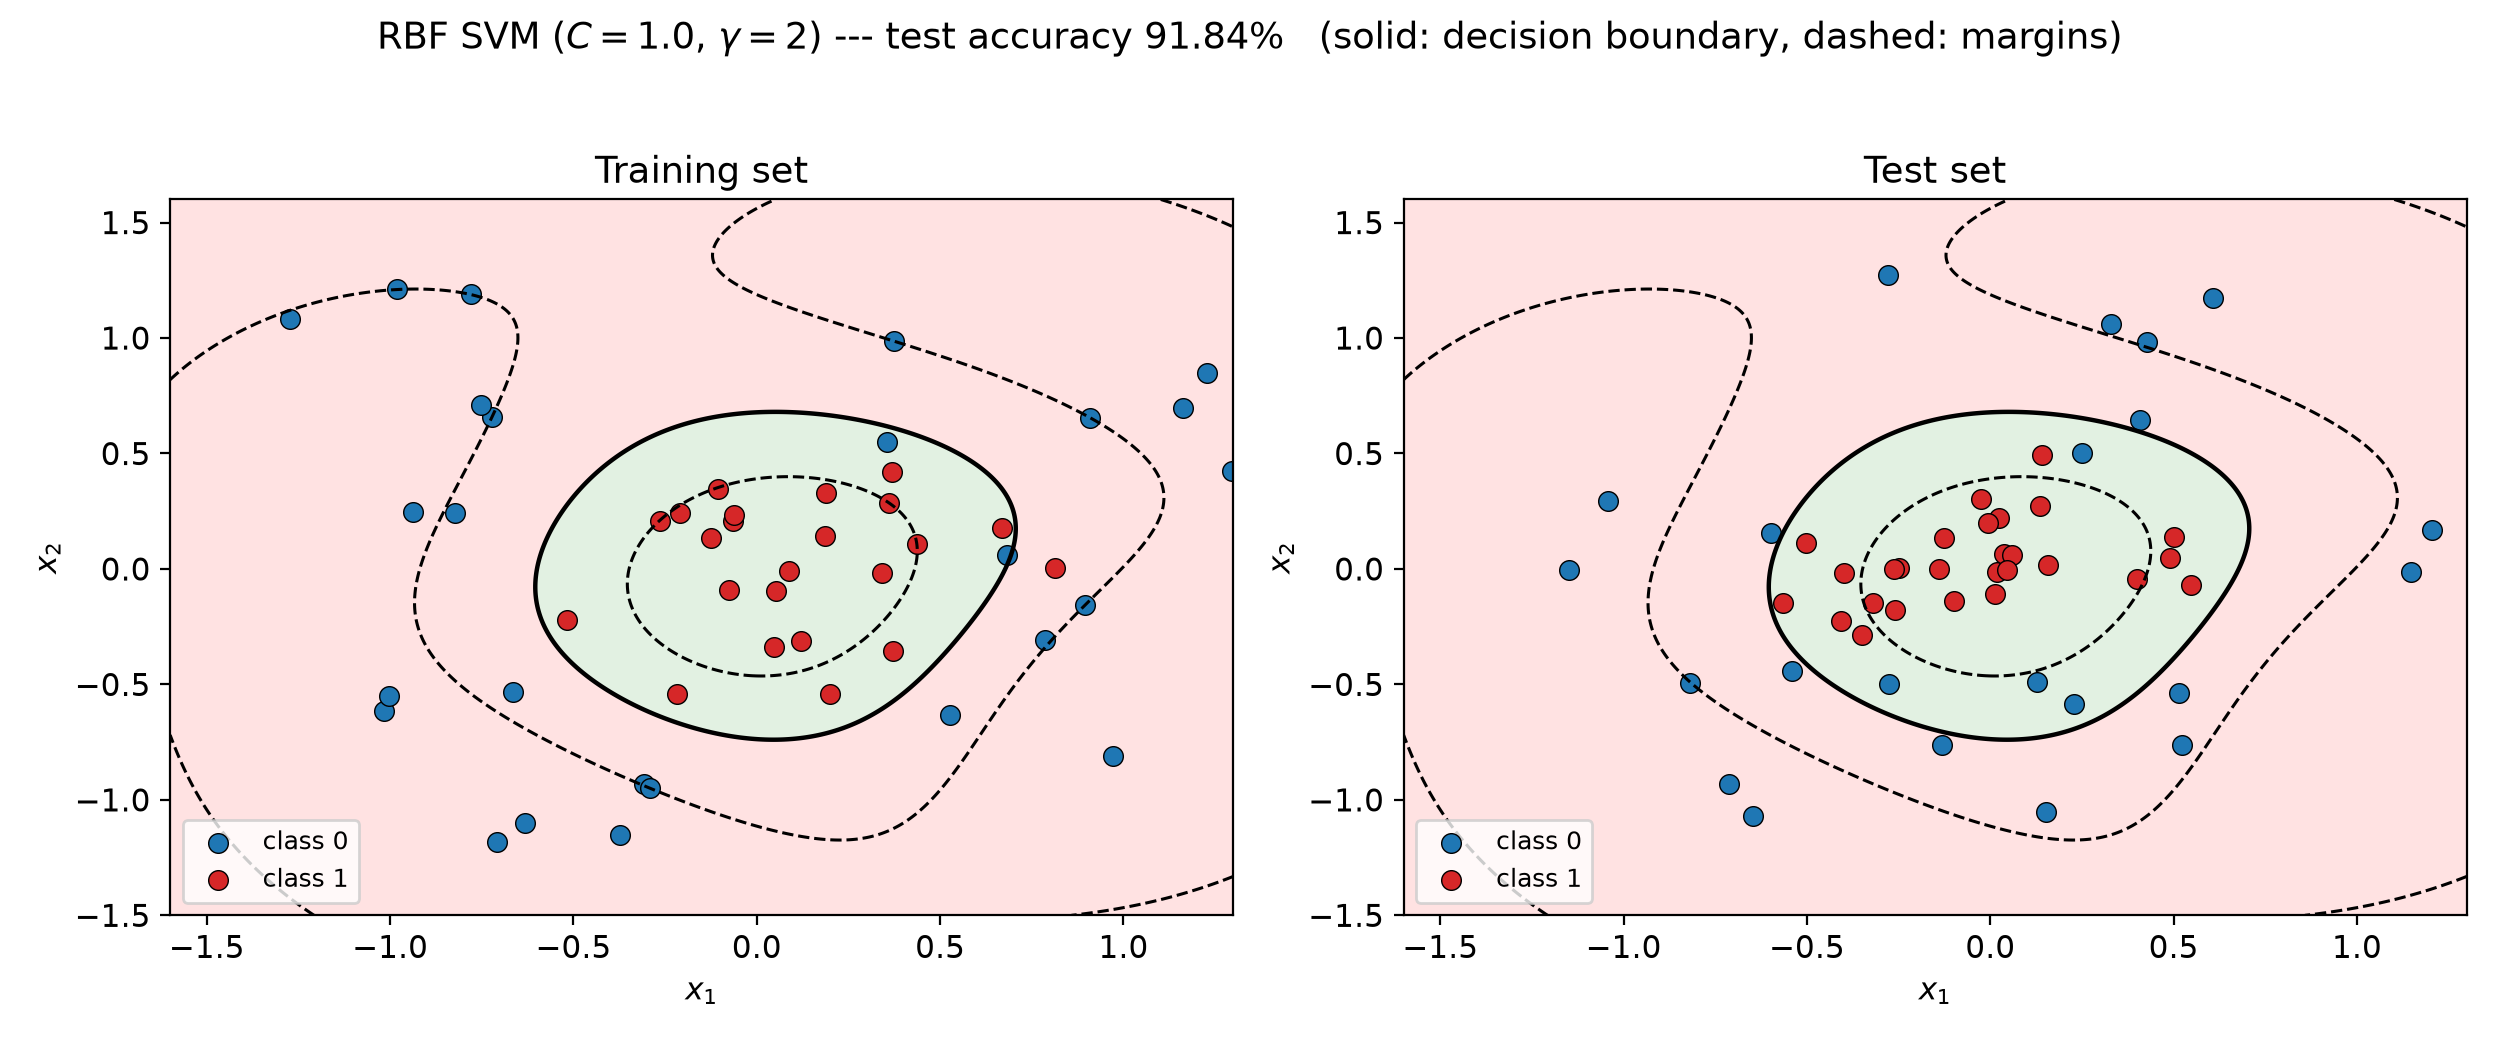
\includegraphics[width=\linewidth]{q2_rbf.png}
\caption*{RBF SVM ($C=1.0$, $\gamma=2$): decision boundary (solid) and margins (dashed) shown on the training set (left) and test set (right). Test accuracy $=91.84\%$.}
\end{figure}

\begin{figure}[h]
\centering
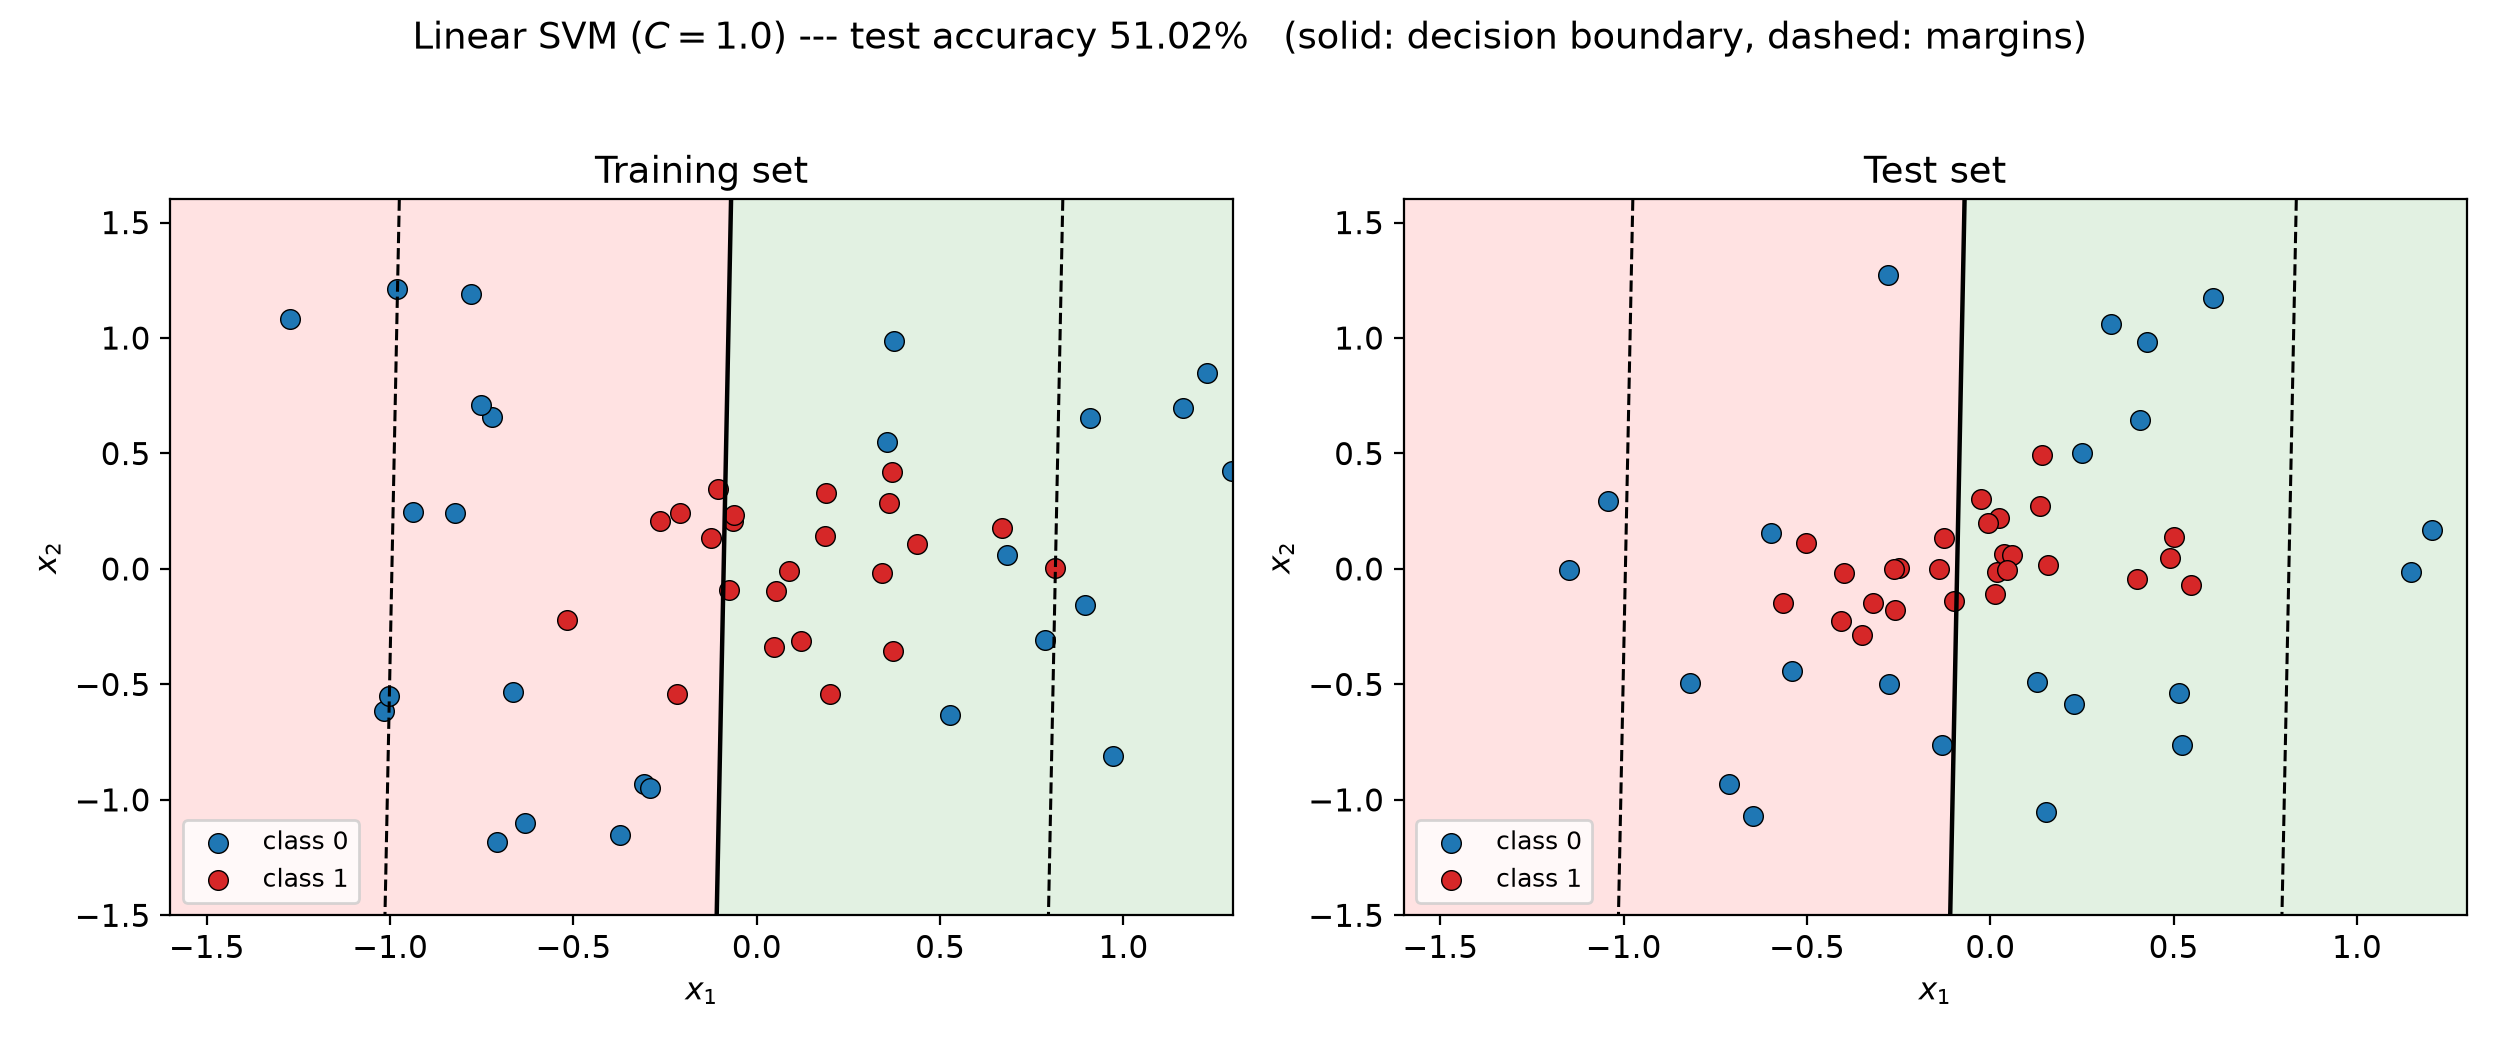
\includegraphics[width=\linewidth]{q2_linear.png}
\caption*{Linear SVM ($C=1.0$): decision boundary (solid) and margins (dashed). Test accuracy $=51.02\%$, matching the example in the assignment.}
\end{figure}

\subsection*{Code}
\begin{lstlisting}[language=Python]
from sklearn.svm import SVC

# Model 1: linear kernel, soft margin
clf_lin = SVC(kernel='linear', C=1.0)
clf_lin.fit(X_train, y_train)
acc_lin = clf_lin.score(X_test, y_test)      # 0.5102

# Model 2: RBF kernel, soft margin
clf_rbf = SVC(kernel='rbf', C=1.0, gamma=2)
clf_rbf.fit(X_train, y_train)
acc_rbf = clf_rbf.score(X_test, y_test)      # 0.9184
print(len(clf_rbf.support_))                 # 23 support vectors
\end{lstlisting}

The full plotting script (decision boundary + margins on both sets) is included as
\texttt{q2\_svm.py}.

%==================================================================
\section*{Question 3: K-means and DBSCAN}

\textbf{Points:}
$a(1,2)$, $b(2,3)$, $c(2,4)$, $d(6,5)$, $e(3,1)$, $f(3,3)$, $g(4,4)$, $h(7,6)$,
$i(8,8)$, $j(8,9)$, $k(9,4)$, $l(5,9)$, $m(4,7)$, $n(6,8)$, $o(6,4)$.

\subsection*{(a) K-means, first iteration}

Initial centres: $\mu_1=(7,4)$, $\mu_2=(3,6)$, $\mu_3=(7,9)$.
Using squared Euclidean distance, assign each point to the nearest centre:

\begin{center}
\begin{tabular}{c|ccccccccccccccc}
\toprule
& $a$ & $b$ & $c$ & $d$ & $e$ & $f$ & $g$ & $h$ & $i$ & $j$ & $k$ & $l$ & $m$ & $n$ & $o$\\
\midrule
$d_1^2$ (to $(7,4)$) & 40 & 26 & 25 & 2 & 25 & 17 & 9 & 4 & 17 & 26 & 4 & 29 & 18 & 17 & 1\\
$d_2^2$ (to $(3,6)$) & 20 & 10 & 5 & 10 & 25 & 9 & 5 & 16 & 29 & 34 & 40 & 13 & 2 & 13 & 13\\
$d_3^2$ (to $(7,9)$) & 85 & 61 & 50 & 17 & 80 & 52 & 34 & 9 & 2 & 1 & 29 & 4 & 13 & 2 & 26\\
\midrule
cluster & 2 & 2 & 2 & 1 & 1 & 2 & 2 & 1 & 3 & 3 & 1 & 3 & 2 & 3 & 1\\
\bottomrule
\end{tabular}
\end{center}

(Ties: $e$ is equally distant from centres 1 and 2 --- assigned to cluster 1 here; the tie can
be broken arbitrarily without changing the following analysis.)

Updated centres after the first iteration:
\begin{align*}
\mu_1^{(1)} &= \text{mean}\{d,e,h,k,o\}
= \bigl(\tfrac{6+3+7+9+6}{5},\ \tfrac{5+1+6+4+4}{5}\bigr) = \boxed{(6.2,\ 4)},\\
\mu_2^{(1)} &= \text{mean}\{a,b,c,f,g,m\}
= \bigl(\tfrac{1+2+2+3+4+4}{6},\ \tfrac{2+3+4+3+4+7}{6}\bigr)
= \boxed{(2.6667,\ 3.8333)},\\
\mu_3^{(1)} &= \text{mean}\{i,j,l,n\}
= \bigl(\tfrac{8+8+5+6}{4},\ \tfrac{8+9+9+8}{4}\bigr) = \boxed{(6.75,\ 8.5)}.
\end{align*}

\begin{figure}[h]
\centering
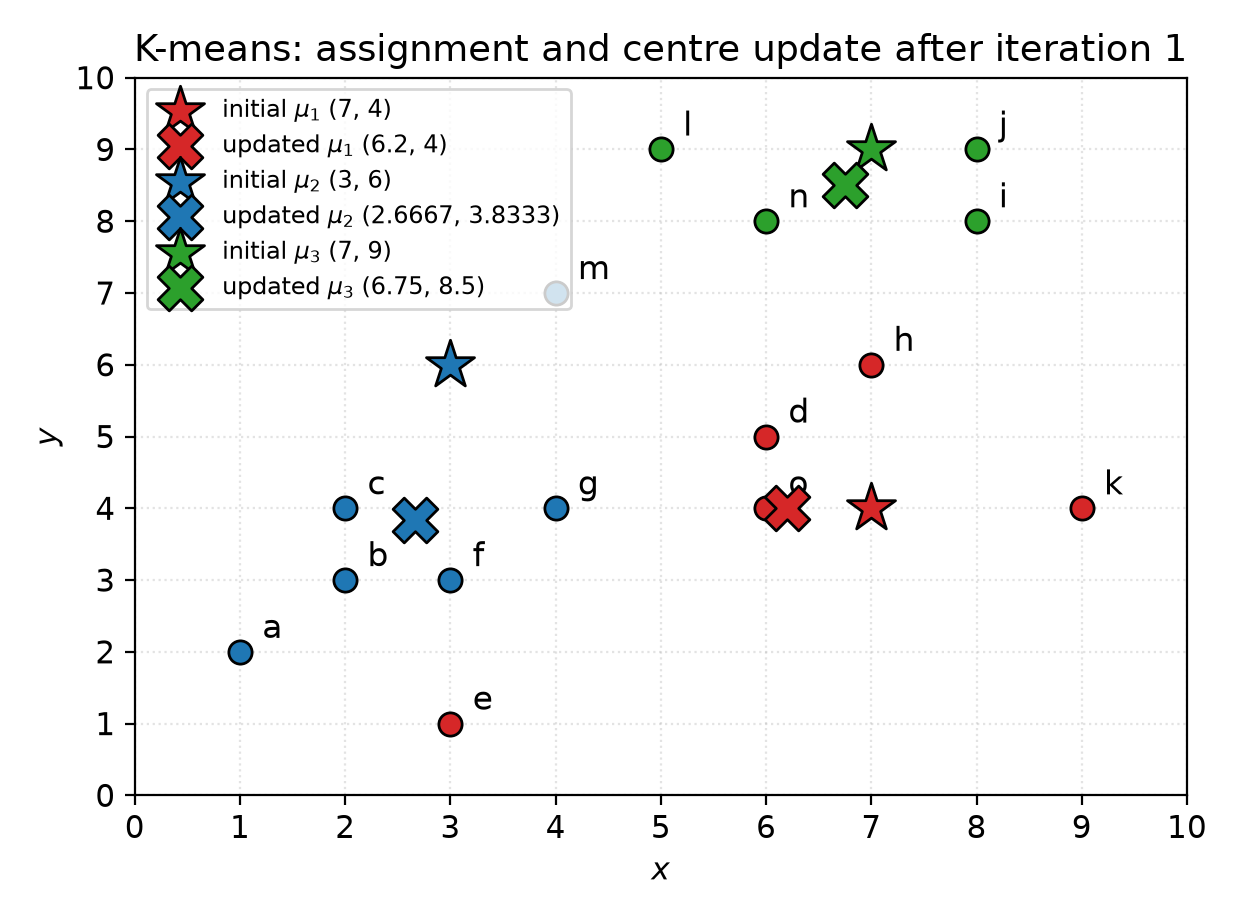
\includegraphics[width=0.75\linewidth]{q3_kmeans.png}
\caption*{Initial centres (stars) and updated centres after iteration 1 (X marks).}
\end{figure}

\subsection*{(b) DBSCAN: $\epsilon=2$, minpts $=3$}

$\epsilon$-neighbourhoods (including the point itself, Euclidean distance):

\begin{center}
\begin{tabular}{clcl}
\toprule
point & $N_\epsilon$ & point & $N_\epsilon$\\
\midrule
$a$ & $\{a,b\}$ & $i$ & $\{i,j,n\}$\\
$b$ & $\{a,b,c,f\}$ & $j$ & $\{i,j\}$\\
$c$ & $\{b,c,f,g\}$ & $k$ & $\{k\}$\\
$d$ & $\{d,h,o\}$ & $l$ & $\{l,n\}$\\
$e$ & $\{e,f\}$ & $m$ & $\{m\}$\\
$f$ & $\{b,c,e,f,g\}$ & $n$ & $\{i,l,n\}$\\
$g$ & $\{c,f,g,o\}$ & $o$ & $\{d,g,o\}$\\
$h$ & $\{d,h\}$ & &\\
\bottomrule
\end{tabular}
\end{center}

\begin{itemize}
\item \textbf{Core points} ($|N_\epsilon|\ge 3$):
$\boxed{b,\ c,\ d,\ f,\ g,\ i,\ n,\ o}$
\item \textbf{Border points} (not core, but within $\epsilon$ of a core point):
$\boxed{a,\ e,\ h,\ j,\ l}$
\item \textbf{Noise points} (neither core nor border): $\boxed{k,\ m}$
\end{itemize}

\subsection*{(c) Is $h$ density-reachable from $b$?}

Yes. Density-reachability requires a chain of points $p_0,\dots,p_k$ with $p_0=b$, $p_k=h$,
where each step goes from a core point to a point in its $\epsilon$-neighbourhood. One such
chain is
\[
\boxed{\ b \to c \to g \to o \to d \to h\ }
\]
Check: $c\in N_\epsilon(b)$, $g\in N_\epsilon(c)$, $o\in N_\epsilon(g)$,
$d\in N_\epsilon(o)$, $h\in N_\epsilon(d)$, and $b,c,g,o,d$ are all core points. Hence $h$ is
density-reachable from $b$.

\subsection*{(d) Density-based clusters}

The core points form two connected components (via direct density-reachability between core
points):
\[
\{b,c,d,f,g,o\}\ \cup\ \text{border }\{a,e,h\}
\qquad\text{and}\qquad
\{i,n\}\ \cup\ \text{border }\{j,l\}.
\]
Therefore
\begin{itemize}
\item Cluster 1: $\boxed{\{a,\ b,\ c,\ d,\ e,\ f,\ g,\ h,\ o\}}$
\item Cluster 2: $\boxed{\{i,\ j,\ l,\ n\}}$
\end{itemize}
and $k,\ m$ remain noise points (not part of any cluster).

%==================================================================
\section*{Question 4: Hierarchical clustering (group average)}

Distance matrix:

\begin{center}
\begin{tabular}{c|ccccc}
\toprule
& A & B & C & D & E\\
\midrule
A & 0 & 8 & 6 & 2 & 1\\
B & 8 & 0 & 7 & 3 & 6\\
C & 6 & 7 & 0 & 9 & 5\\
D & 2 & 3 & 9 & 0 & 4\\
E & 1 & 6 & 5 & 4 & 0\\
\bottomrule
\end{tabular}
\end{center}

Group average distance between clusters $U,V$:
$d(U,V)=\frac{1}{|U||V|}\sum_{u\in U}\sum_{v\in V} d(u,v)$.

\paragraph{Iteration 1.} Smallest distance is $d(A,E)=1$. Merge $A$ and $E$ into $AE$
($d=1$). Updated table:
\begin{center}
\begin{tabular}{c|cccc}
\toprule
& AE & B & C & D\\
\midrule
AE & 0 & $(8{+}6)/2=7$ & $(6{+}5)/2=5.5$ & $(2{+}4)/2=3$\\
B & 7 & 0 & 7 & 3\\
C & 5.5 & 7 & 0 & 9\\
D & 3 & 3 & 9 & 0\\
\bottomrule
\end{tabular}
\end{center}

\paragraph{Iteration 2.} Smallest distances: $d(B,D)=3$ and $d(AE,D)=3$ (tie; tie-breaking
does not affect the final structure). Merge $B$ and $D$ into $BD$ ($d=3$). Updated table:
\[
d(AE,BD)=\frac{8+6+2+4}{4}=\frac{20}{4}=5,
\qquad
d(C,BD)=\frac{7+9}{2}=8,
\qquad
d(C,AE)=5.5 .
\]
\begin{center}
\begin{tabular}{c|ccc}
\toprule
& AE & BD & C\\
\midrule
AE & 0 & 5 & 5.5\\
BD & 5 & 0 & 8\\
C & 5.5 & 8 & 0\\
\bottomrule
\end{tabular}
\end{center}

\paragraph{Iteration 3.} Smallest distance is $d(AE,BD)=5$. Merge into $AEBD$ ($d=5$).
Updated table:
\[
d(C,AEBD)=\frac{6+5+7+9}{4}=\frac{27}{4}=6.75 .
\]
\begin{center}
\begin{tabular}{c|cc}
\toprule
& AEBD & C\\
\midrule
AEBD & 0 & 6.75\\
C & 6.75 & 0\\
\bottomrule
\end{tabular}
\end{center}

\paragraph{Iteration 4.} Merge $AEBD$ and $C$ into the single cluster $ABCDE$ at $d=6.75$. Done.

\begin{figure}[h]
\centering
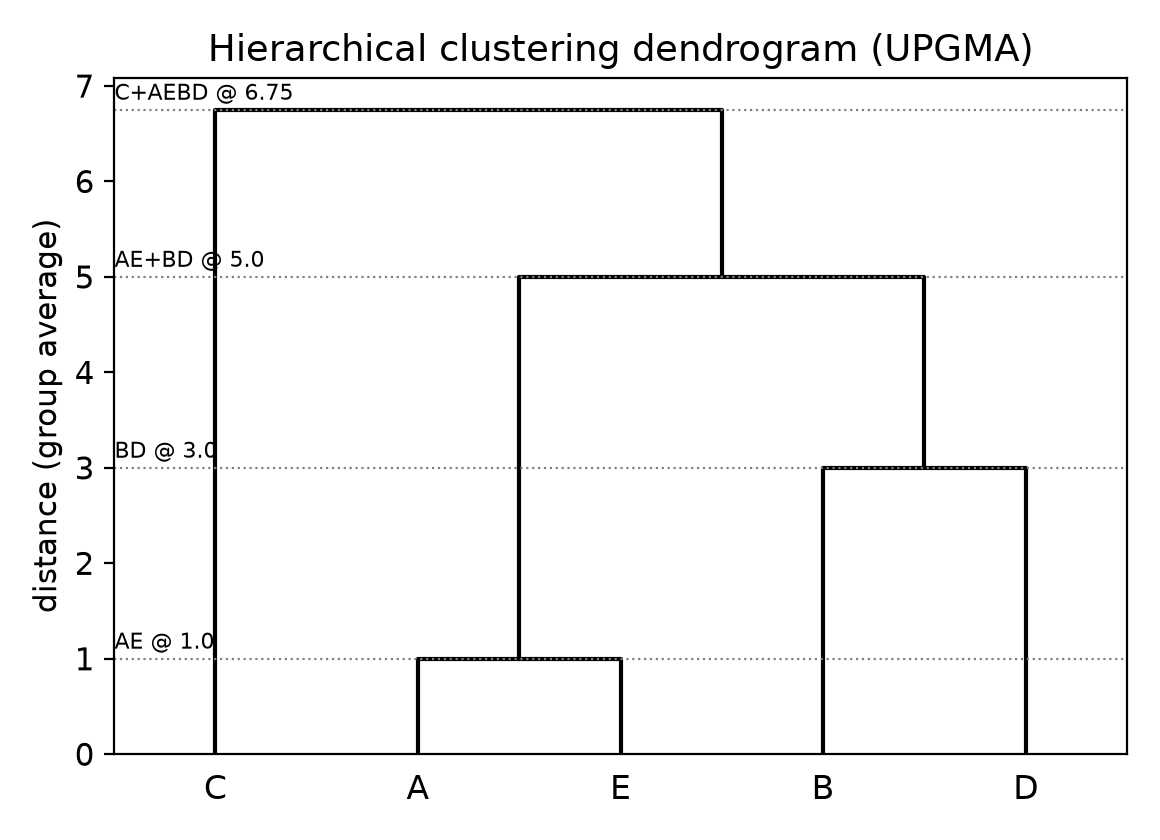
\includegraphics[width=0.8\linewidth]{q4_dendrogram.png}
\caption*{Final dendrogram. Merge order: $A$--$E$ at 1, $B$--$D$ at 3, $AE$--$BD$ at 5, then
$C$ joins at 6.75.}
\end{figure}

\textbf{Summary of the merges (order in which points are merged):}
\[
\boxed{\ (A,E)\xrightarrow{1.0}\ (B,D)\xrightarrow{3.0}\ (AE,BD)\xrightarrow{5.0}\ (AEBD,C)\xrightarrow{6.75}\ }
\]

\end{document}
